\begin{frame}
    \frametitle{Final Products}
    \hspace*{-1cm}
    \fbox{\begin{minipage}[t]{0.4\paperwidth}
        \centering
        \textbf{Meteor Observations}
        \begin{columns}
            \begin{column}{0.35\linewidth}
                {\setbeamercovered{transparent=60}\noindent
                \begin{itemize}
                    \footnotesize
                    \item<0> Position
                    \item<0> Time
                    \item<0> Speed
                \end{itemize}}
            \end{column}
            \begin{column}{0.6\linewidth}
                {\setbeamercovered{transparent=60}\setlength{\leftmargini}{0pt}
                \begin{itemize}
                    \footnotesize
                    \item<0> Radial wind
                    \item<0> Diffusion coefficient
                    \item<0> Mass
                    \item<0> Trail orientation
                \end{itemize}}
            \end{column}
        \end{columns}
        \(\times1,000 +\) observations per hour... 
        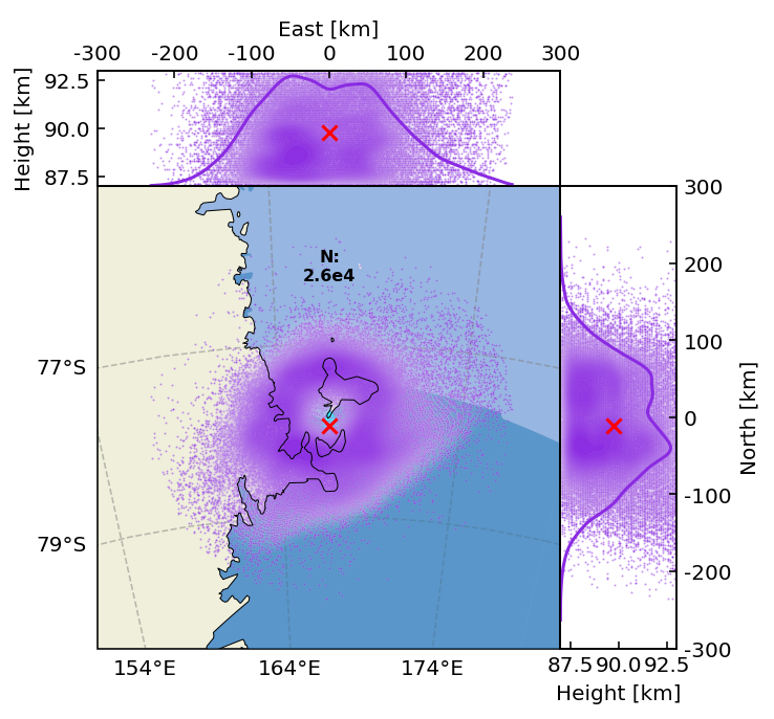
\includegraphics[width=0.8\linewidth]{img/mcmurdo_ortho.png} 
    \end{minipage}}%
    \begin{minipage}[t]{0.6\paperwidth}
        {\(\xrightarrow[Analyze]{Combine}\)}\uncover<2->{\textbf{\ \ Science}}
    \end{minipage}
    \begin{tikzpicture}[remember picture, overlay]
        \node<2->[anchor=south east] (image) at ([xshift=-0.5cm, yshift=0.5cm + 3cm + 5pt]current page.south east) {
            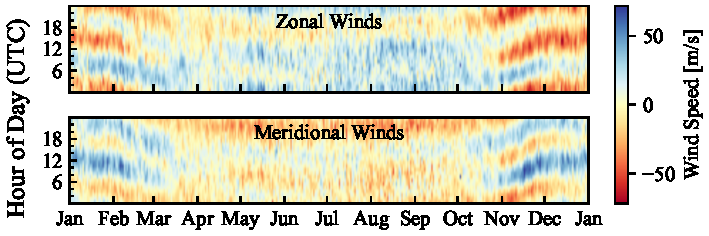
\includegraphics[width=5.5cm]{img/seasonal_trends.pdf}
        };
        \node<2-> at (image.center) {%
            \begin{tcolorbox}[width = 3cm, center, boxrule=0pt,colback=yellow,arc=0pt,auto outer arc,left=0pt,right=0pt,boxsep=0pt]
                \centering
                \footnotesize
                Wind time series
            \end{tcolorbox}
        };
        \node<2->[anchor=south east] (image) at ([xshift=-6.25cm - 5pt, yshift=0.5cm + 3.25cm + 5pt]current page.south east) {
            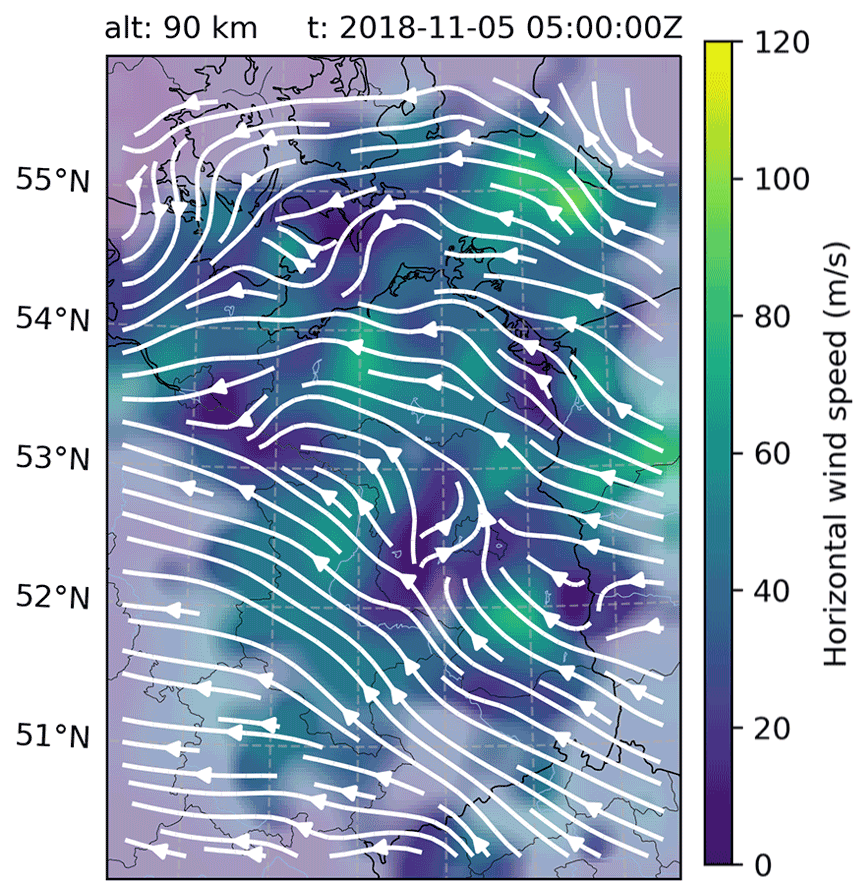
\includegraphics[width=2.5cm]{img/volz_2021.png}
        };
        \node<2-> at (image.center) {%
            \begin{tcolorbox}[width = 2cm, center, boxrule=0pt,colback=yellow,arc=0pt,auto outer arc,left=0pt,right=0pt,boxsep=0pt]
                \centering
                \footnotesize
                Wind maps
            \end{tcolorbox}
        };
        \node<2->[anchor=south east] at ([yshift=0cm, xshift=-0.5cm]image.south east) {%
            {\fontsize{3}{3.4}\selectfont \textcolor{white}{Credit: \citeauthor{volz_FourdimensionalMesosphericLower_2021}, \citeyear{volz_FourdimensionalMesosphericLower_2021} \cite{volz_FourdimensionalMesosphericLower_2021}}}
        };
        \node<2->[anchor=south east] (image) at ([xshift=-3.5cm - 5pt, yshift=0.5cm]current page.south east) {
            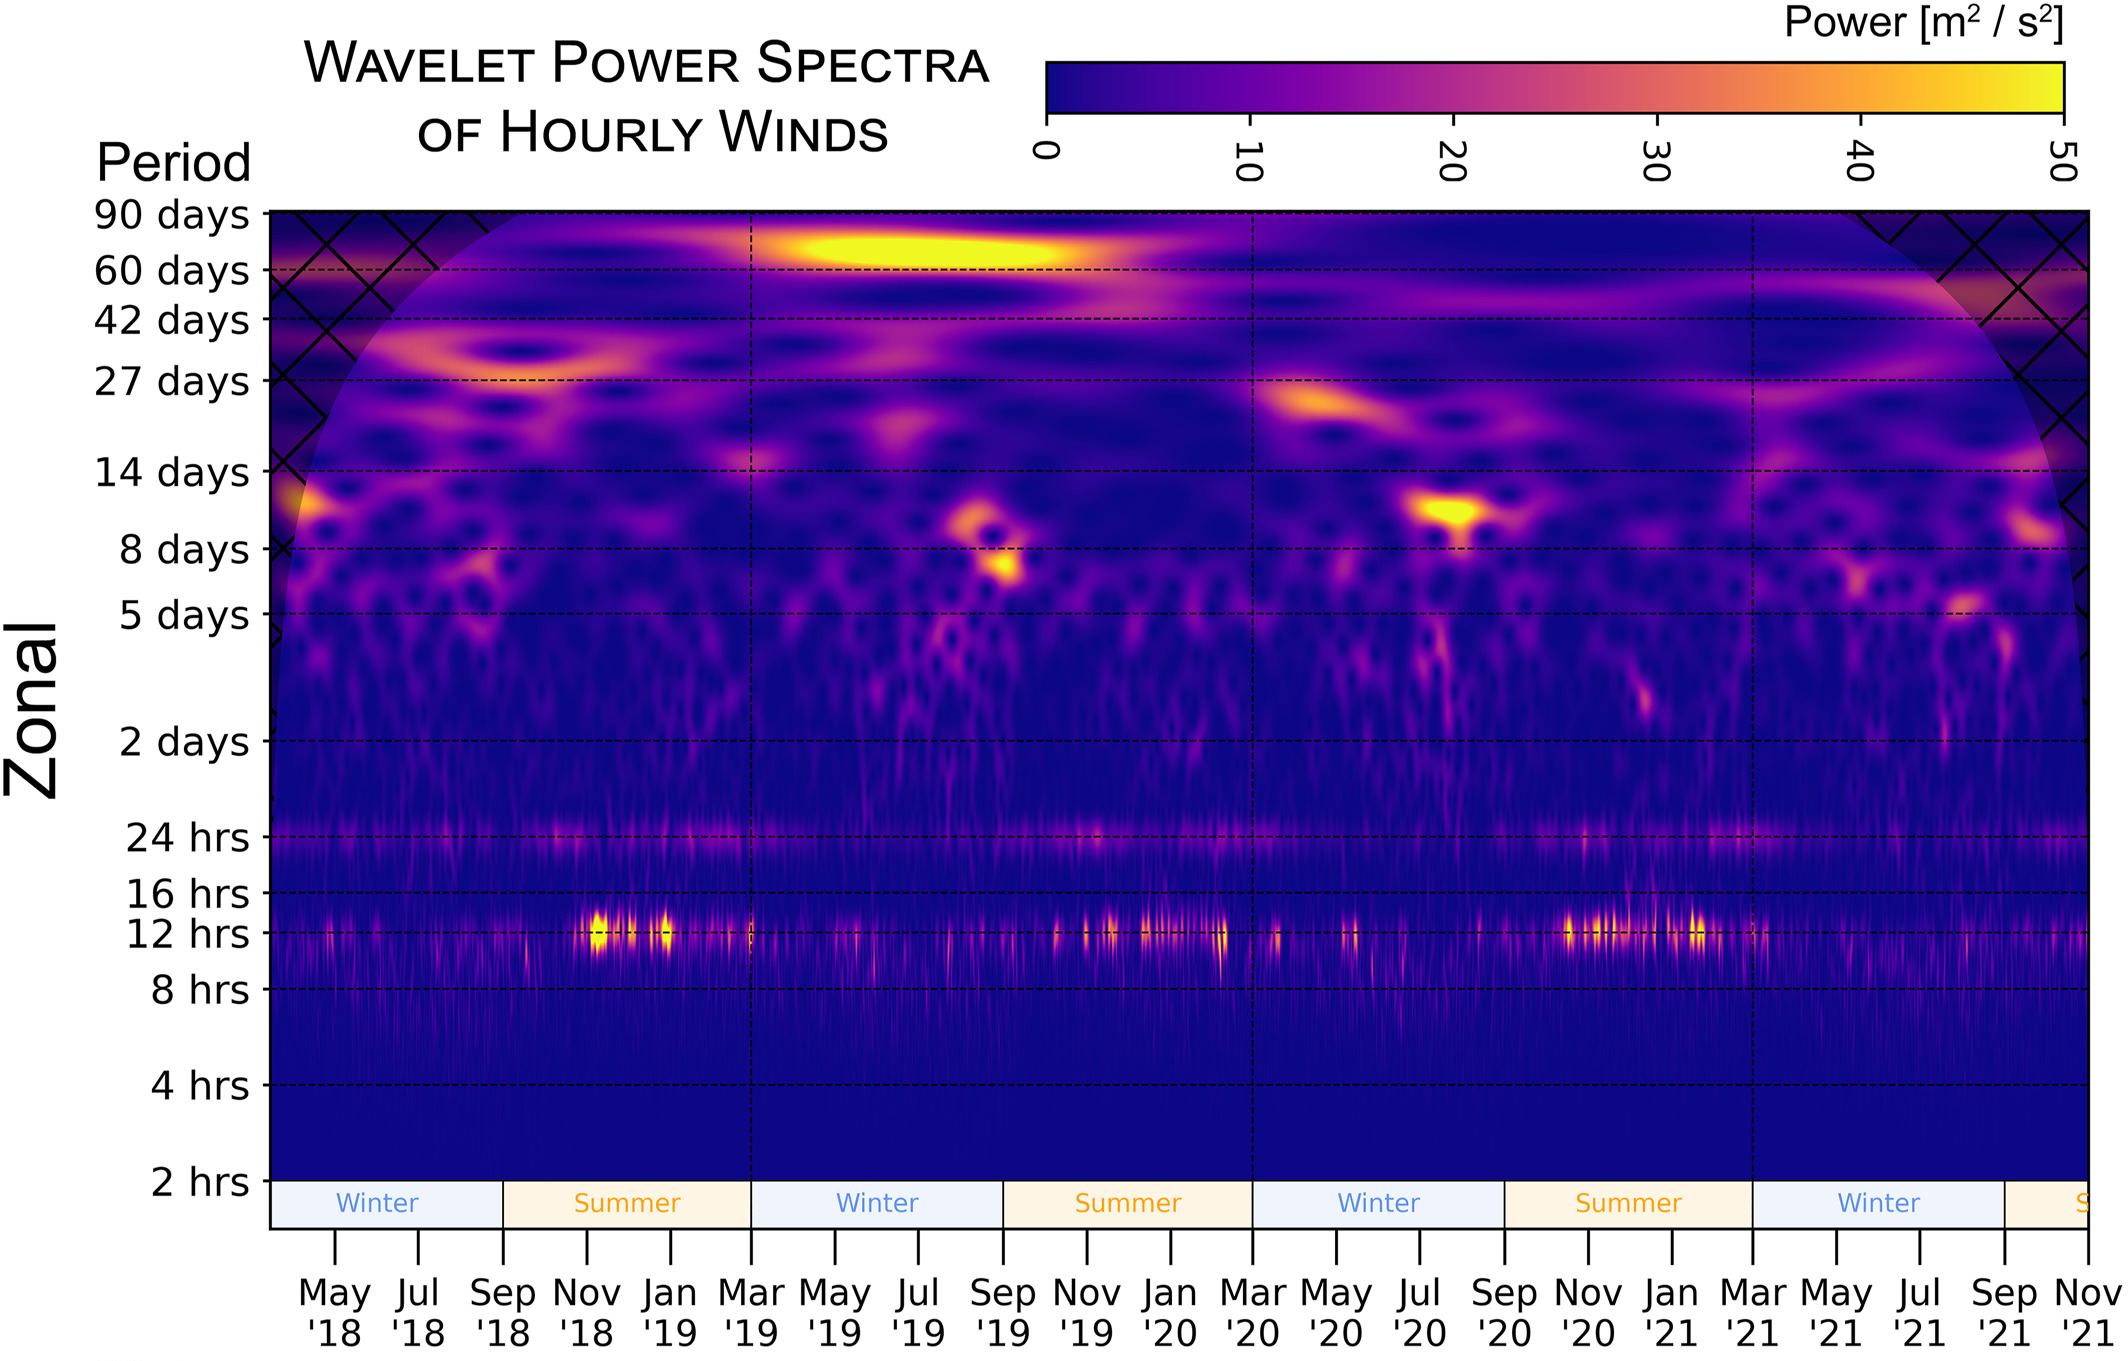
\includegraphics[width=5cm]{img/mcmurdo_wavelet.png}
        };
        \node<2-> at ([xshift=0.25cm, yshift=0.5cm]image.center) {%
            \begin{tcolorbox}[width = 3cm, center, boxrule=0pt,colback=yellow,arc=0pt,auto outer arc,left=0pt,right=0pt,boxsep=0pt]
                \centering
                \footnotesize
                Atmospheric tide temporal analysis
            \end{tcolorbox}
        };
        \node<2->[anchor=south east] at ([yshift=0.5cm, xshift=-0.1cm]image.south east) {%
            {\fontsize{3}{3.4}\selectfont \textcolor{white}{Credit: \citeauthor{marino_FirstObservationsNew_2022}, \citeyear{marino_FirstObservationsNew_2022} \cite{marino_FirstObservationsNew_2022}}}
        };
        \node<2->[anchor=south east] (image) at ([xshift=0cm, yshift=0.5cm]current page.south east) {
                \adjincludegraphics[width=3.5cm,trim={{.5\width} 0  0 {.12\height}},clip]{img/12h_z_90pm2km_15d_results.pdf}};
        \node<2-> at (image.center) {%
            \begin{tcolorbox}[width = 3cm, center, boxrule=0pt,colback=yellow,arc=0pt,auto outer arc,left=0pt,right=0pt,boxsep=0pt]
                \centering
                \footnotesize
                Atmospheric tide spatial analysis
            \end{tcolorbox}
        };
        \node<2->[anchor=south east] (image) at ([xshift=0cm, yshift=0.5cm + 4.5cm + 5pt]current page.south east) {
            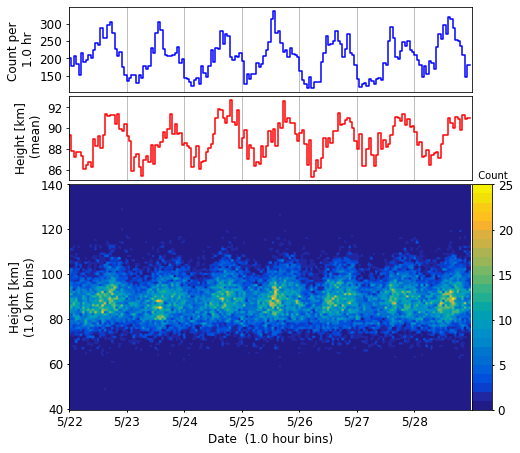
\includegraphics[width=3.5cm]{img/meteor_stats.png}
        };
        \node<2-> at (image.center) {%
            \begin{tcolorbox}[width = 3cm, center, boxrule=0pt,colback=yellow,arc=0pt,auto outer arc,left=0pt,right=0pt,boxsep=0pt]
                \centering
                \footnotesize
                Meteor statistics
            \end{tcolorbox}
        };
        \node<2-> at ([xshift=-3.25cm, yshift=-0.5cm]image.center) {%
            \begin{tcolorbox}[width = 2cm, center, boxrule=0pt,colback=yellow,arc=0pt,auto outer arc,left=0pt,right=0pt,boxsep=0pt]
                \centering
                \footnotesize
                \textit{...and more!}
            \end{tcolorbox}
        };
    \end{tikzpicture}
\end{frame}